\chapter{Background}
\label{chap:related_work}

This thesis' contributions are built on the idea that intrusion tolerance is the last resort, to the best of our knowledge, to build secure and dependable systems.
In this chapter, we present the reasons why we need intrusion tolerance, and then we describe the most relevant related works in the different intrusion tolerance areas.


\section{The Need for Intrusion Tolerance}
The realistic way to provide security is to build mechanisms that protect highly vulnerable systems from powerful attackers.
This is particularly important when considering critical systems that attract highly motivated attackers. 
Then, there is a need to focus on designing mechanisms to make systems safe and resilient despite their number of vulnerabilities and the attacker's power.
In the following, we make an overview of the different approaches that can be combined to deal with the challenge of providing security and dependability for critical systems.

\subsection{Vulnerabilities Prevention}
One of the primary techniques to impede attackers' success is to try to avoid that vulnerabilities persist in the code throughout all the software development phases until it is in production. 
One way to do that is to detect and remove vulnerabilities during the development and testing stages.
We can identify a few standard techniques that are used to prevent the existence of vulnerabilities: static, dynamic, concolic analysis, and vulnerability workarounds.

A few examples of static analysis are source code verification and validation. 
However, the most common techniques typically over-simplify the protocols to make them formally verifiable or just use very particular version to verify~\cite{Klein:2009,Nelson:2017}. 
Moreover, this process consumes much time, and it is expensive for most of the companies, which makes this method difficult to scale to complex systems~\cite{Giuffrida:2013}.
For example, an \gls{os} kernel was formally verified~\cite{Klein:2009}, but contrary to the Linux kernel that has more than 20 million lines of code\footnote{Source: https://www.linuxcounter.net/statistics/kernel on 2nd July 2018} this only has 10k lines of code.

Fuzzing is a dynamic technique and its success in finding vulnerabilities or bugs results from a good set of input test cases.
These can be built manually and tuned for a particular application, or randomly generated, for the latter they are likely to fail on triggering more complex vulnerabilities.
Another dynamic technique, which is used in information security, is taint analysis.
In this technique, any program variable that can be modified by a user is seen as a vulnerability trigger. 
Then, when it is accessed, it becomes tainted for further inspection.
The main limitations of taint analysis are that vulnerabilities are detected only for the execution paths that have been explored by the tester, and it is limited to call/return functions being challenging to cover shared memory or global variables~\cite{Yamaguchi:2015}.

Concolic testing is a technique that performs symbolic execution along with a concrete execution path. 
Therefore, it is more accurate than fuzzing, but it tends to succumb to path explosion.
Some of these techniques can be combined to take the best of some of the approaches described before (e.g., using fuzzing with symbolic execution~\cite{Stephens:2016}).

Finally, some works propose vulnerability workarounds that intend to minimize the vulnerable window between vulnerability disclosure and the patch release.
Typically, these solutions have two phases: first, the detection phase where they look for vulnerabilities in the source code, and a second, where they instrument the code with the vulnerability workaround.
Although they may have good coverage of the vulnerabilities, there are a few caveats on applying such solution.
For example, some workarounds may crash the application upon the vulnerability activation, or they may disable the main functions that clients use in the software~\cite{Huang:2016}, i.e., compromising the availability. 
Nevertheless, these are initial steps towards more robust solutions.

\subsection{Fault Detection and Removal}
Most of the previously described techniques work offline and are not complete. 
Therefore, unknown vulnerabilities may arise when the system is already online, allowing the system to be compromised.
Then, we need a more complex approach to cope with the existence of vulnerabilities that can be exploited.
The detection and removal approach works by detecting intrusions, and then trigger a recovery mechanism to clear the resulting fault effects. 
Since some attacks use a combination of different vulnerabilities, which isolated would be harmless, it is hard to detect them when the system is in production. 
This approach presents three problems: 
First, there are no perfect intrusion detectors, and then, stealth attacks may not be detected; 
Second, the service can experience some periods of unavailability while the service is recovering; 
Finally, recovering a system might clean its faults, but the system remains vulnerable.
Therefore, it is easy for an attacker to repeat the same procedure to compromise the system every time it recovers.


\subsection{Fault Tolerance and Masking}
The previously described approaches assume that vulnerability prevention is complete to some extent or that is possible to detect all the attacks.
However, these assumptions are unrealistic, and it is not advisable to trust the security and dependability of a system in a single component, as it creates a single point-of-failure. 
Thus, once the system becomes compromised the whole infrastructure becomes exposed to more attacks. 
The established way to provide a system with tolerance and masking properties is to distribute it to a set of replicas, which execute the same commands in the same order. 
Primary-backup replication (i.e., $1 + 1$ replicas), would suffice if only crash faults are considered. 
If one of the replicas crashes, the other can replace it and deliver the requests correctly.
However, if arbitrary faults are considered, primary-backup replication is not enough because compromised replicas could deliver arbitrary outputs, impeding a client to decide which output is correct.

\gls{smr}~\cite{Lamport:1984} is an active approach that has been employed to ensure fault tolerance~\cite{Schneider:1990} of fundamental services in modern internet-scale infrastructures (e.g.,~\cite{Hunt:2010,Calder:2011,Corbett:2013}).
\gls{smr} is achieved in distributed systems that run an agreement protocol that guarantees that all the replica nodes (i) start from the same state, (ii) execute the same sequence of messages, and (iii) execute the same state transitions. 
These properties guarantee that a service runs deterministically in the distributed replicas.
However, \gls{smr} does not provide tolerance for malicious (Byzantine) faults.
Therefore, one must resort to intrusion tolerance techniques~\cite{Verissimo:2003} to address these more complex type of faults.
Intrusion tolerance was first proposed by Fraga and Powell in 1985~\cite{Fraga:1985} as a solution to address faults without compromising the security of a system. 
More formally, we adopt the following intrusion tolerance definition: 

\begin{defn}
\emph{``A replicated intrusion-tolerant system is a replicated system in which a malicious adversary needs to compromise more than $f$ out-of $n$ components in less than $T$ time units to make it fail.''}~\cite{Bessani:2011}
\label{def:def2}
\end{defn}

It is necessary to employ \gls{bft} \gls{smr}, a particular case of \gls{smr}, to build a system capable of operating correctly even in the presence of some compromised nodes.
Since no single replica can be trusted completely, the correctness of the system comes from the majority of correct nodes. 


Although \gls{bft} protocols provide safety to a bound of $f$ faulty nodes, with sufficient time, i.e., greater than $T$, an adversary eventually compromises $f+1$ nodes.
Then, additional mechanisms are needed to clean the faulty state (e.g., from time to time the nodes are recovered~\cite{Castro:2002}).
However, if a recovered node remains vulnerable to the same attack, the time to compromise $f+1$ replicas becomes smaller as the attacker already knows how to exploit those vulnerabilities.
For this reason, several authors have built their models assuming that nodes fail independently due to some mechanism that provides failure independence (e.g.,~\cite{Castro:2002,Bessani:2008,Veronese:2013,Sousa:2010}).
For instance, to increase the time or effort $T$ that takes to compromise $f+1$, one must employ recoveries to reset the replicas' faulty state. 
Moreover, to avoid reintroducing replicas with the same vulnerabilities in the system, the recovery should change the replica's code somehow.
Finally, such mechanism needs careful management otherwise the decisions are made with no criteria which could decrease $T$ after all.
In the following sections, we present and describe several works on specific areas of intrusion tolerance.


\section{Byzantine Fault Tolerance}

\side{OSDI 1999}
Castro and Liskov’s \textsc{Pbft}~\cite{Castro:1999} was the first Practical \gls{bft} replicated system, and it was initially proposed as a solution to handle Byzantine faults of both accidental and malicious nature.
The correctness of a \gls{bft} service arises from the existence of a quorum of correct nodes capable of reaching consensus on the (total) order of messages to be delivered to the replicas.
For instance, to tolerate a single replica failure, the system typically must have four replicas. 
\textsc{Pbft} implements a \gls{smr} protocol that guarantees both liveness and safety for $\lfloor\frac{n-1}{3}\rfloor$ out of a total of $n$ replicas are simultaneously faulty. 
These properties hold even in asynchronous systems such as the internet. 
\textsc{Pbft-pr} implements a \gls{smr}, therefore, it must guarantees that each replica executes the same commands, in the same order, and then it produces the same output. 
In Figure~\ref{fig:bft} we present an overview of \textsc{Pbft} protocol that can be summarized as follows:
A client \emph{(c)} sends a message to all the replicas \emph{(R1-R4)}.
Then, the leader replica has to assign a sequence number to the request and multicast a pre-prepare message to the other replicas. 
If the replicas agree with the leader, they send a prepare message to each other. 
At this phase of the protocol, every correct replica agrees on the ordering of the messsages.  
Every replica sends a commit message. 
When a replica receives the commit message from a quorum, it executes the message. 
In the end, it replies to the client. 
Every replica shares a key with each other and with clients. These keys are used to authenticate messages with a \gls{mac}. 
The messages that are multicast by the clients are authenticated with a vector of \glspl{mac}. 
Then, each replica verifies its own \gls{mac}.
The authors validated this \gls{bft} library implementing a Byzantine fault-tolerant filesystem. 
The results show that when the workload increases the throughput and latency is nearly the same as a non-replicated system. 

\begin{figure}[h]
\begin{center}
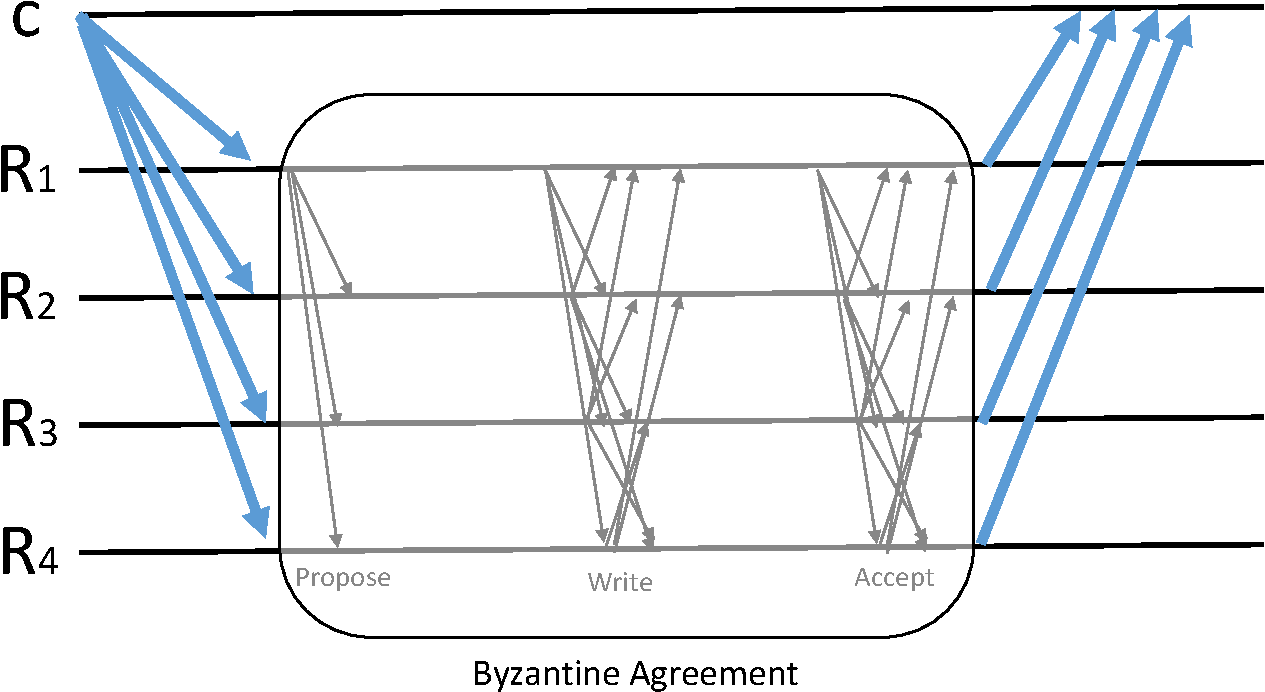
\includegraphics[width=.7\columnwidth]{images/images/bft.pdf}
\caption{Byzantine Fault Tolerance protocol overview.}
\label{fig:bft}
\end{center}
\end{figure}

The \textsc{Pbft} performance encouraged the use of \gls{bft} in common systems, and to develop optimizations to improve \gls{bft} protocols. 
Since the \textsc{Pbft-pr} proposal, some work has been dedicated to improve \gls{bft} protocols (see Table~\ref{tab:bft}):


\begin{table}[h]
\begin{center}
{\footnotesize
\begin{tabular}{ p{2.5cm}  p{10.0cm}  }\hline
\textsc{Zyzzyva}~\cite{Kotla:2010}  & Introduces speculation to avoid the expensive three phase commit before processing the requests. This might introduce some inconsistency in the state of the replicas when speculation fails, and the client needs to help replicas to fix the servers’ inconsistency. \\ \hline            
\textsc{Upright}~\cite{Clement:2009} & It provides a straightforward way to also add BFT to crash fault tolerant systems. \\ \hline    
\textsc{Aardvark}~\cite{Clement:2009b} & Shifts the paradigm to a new design. This design improves the performance under faulty scenarios trading some performance on the normal case. \\ \hline
\textsc{BFT-SMaRt}~\cite{Bessani:2014} & It is modular and multicore-aware. Supports replica reconfiguration and has a flexible programming interface. \\ \hline
\textsc{COP}~\cite{Behl:2015} & It is the most recent BFT implementation that reached 2.4 million operations per second. This was achieved mostly due to BFT architecture changes.\\  \hline  
\end{tabular}
}
\caption{Brief overview of the most relevant BFT works.}

\label{tab:bft}
\end{center}
\end{table}




\paragraph{Summary.} 

In this thesis, we propose a control plane for \gls{bft} systems, hence \gls{bft} systems have significant importance in this work.
They play an essential part as they guarantee that replicas execute correctly while tolerating malicious failures in a subset of the replicas.
The implementation of such \gls{bft} protocol is a complex task, mainly if we need to include mechanisms for state transfer, reconfiguration, and guarantee a good performance.
Therefore, we prefer to rely on existent libraries than to build a new one.
Nevertheless, for some contributions (see Chapter~\ref{chap:sieveq}) we needed to perform some modifications on the chosen library.

\side{Zyzzyva TOCS 2010, UpRight SOSP 2009, Aardvark NSDI 2009, BFT-SMART DSN 2014, COP Middleware 2015} 


\section{Replica Rejuvenation}
\side{International Symposium on Fault-Tolerant Computing 93, 95}
Software rejuvenation was proposed in the 90's~\cite{Huang:1993,Huang:1995} as a proactive approach to prevent performance degradation and failures due to software aging. 
This solution was implemented using three components: a watchdog process (\texttt{watchd}), a checkpoint library (\texttt{libft}) and a replication mechanism (\texttt{REPL}). 
A primary node executes the application and also runs the \texttt{watchd} to monitor the application crashes and hangs. 
The backup node, while its application is inactive, keeps on monitoring the primary node. 
Additionally, there is a routine (provided by \texttt{libft}) that periodically makes checkpoints and logging. 
These checkpoints are replicated with \texttt{REPL} in the backup node. 
When the primary node crashes or hangs, it is restarted, and if needed the backup takes his place on the execution.



Only some years later, proactive recovery was adopted on \gls{bft} replicated systems by Castro and Liskov~\cite{Castro:2002}.\side{TOCS 2002}
In order to support long-running services, they introduced the notion of proactive recovery for \gls{bft} services. 
The objective is to rejuvenate replicas periodically to remove stealth attackers and support the execution of long-running services. 
This mechanism allows that an adversary control up to $f$ replicas before a recovery.
Moreover, \textsc{Pbft-pr} introduces additional mechanisms to guarantee that \gls{smr} properties are maintained even with recoveries.
In particular, a \emph{state transfer} protocol, which allows that recovered replicas fetch a correct and up to date state from the other (correct) replicas.
Additional assumptions are needed to guarantee the \textsc{Pbft-pr}'s liveness and safety during the recoveries: 
(i) Each replica contains a trusted chip to store its private key, and it can sign and decrypt messages without revealing the key; 
(ii) The replicas' public keys are stored in a read-only memory, which needs physical access to be modified; 
And (iii) a watchdog timer is used to avoid human interaction to restart replicas. 
The watchdog hands the execution to the recovery monitor, which cannot be interrupted.


Zhou~\etal{}~\cite{Zhou:2002} presented \textsc{Coca}, a fault-tolerant online certification authority to be deployed both in a local area network and on the internet.\side{TOCS 2002}
It employs proactive recoveries to refresh replicas' state (e.g., faulty or incorrect states) as to refresh the private keys of the replicas.
The authors implemented \textsc{Coca} in Byzantine quorum systems as they do not require timing assumptions.
Moreover, and contrary to \textsc{Pbft-pr}, it does not rely on trusted components.
From these model decisions, \textsc{Coca} may need a trusted administrator to refresh the server keys.
However, and more importantly, the asynchronous model may compromise the safety (i.e., $f$ faulty nodes in-between recoveries) as it was shown by Sousa~\etal{}~\cite{Sousa:2007}. 
Sousa~\etal{} stated the need for hybrid-systems that require some level of synchrony to guarantee safety and liveness of such systems.


Reiser and Kapitza~\cite{Reiser:2007} and Distler~\etal{}~\cite{Distler:2008} identified virtualization as a useful mechanism to implement proactive recovery. \side{Workshops 2007 2008}
They proposed an architecture, named \textsc{VM-FIT}, that is divided into two domains: an untrusted domain and a trusted domain.
The intrusion-tolerant replicated system executes in the untrusted domain, running in \gls{vm}. 
While \textsc{VM-FIT} executes in a trusted domain, i.e., in the \gls{vmm}. 
Virtualization provides isolation between the untrusted and the trusted domains. 
Therefore, it can trigger recoveries from the trusted domain in a synchronous manner. 
Moreover, virtualization reduces downtime of the service during the recovery and makes the state transfer between replicas more efficient. 
The authors implemented this system using the Xen hypervisor to implement both domains: the trusted domain is the Xen Dom0, and the replicas run in the untrusted domains, DomUs.

Sousa~\etal{}~\cite{Sousa:2010} improved the state-of-the-art recovery algorithms by introducing \gls{prrw}. \side{TPDS 2010}
It removes the effects of faults ``immediately''. 
\textsc{\gls{prrw}} accelerates the rejuvenation process by detecting the faulty replicas behavior and forcing them to recover without sacrificing periodic rejuvenations. 
This type of technique can only be implemented with synchrony assumptions as the recoveries are time triggered~\cite{Sousa:2005}. 
To address this need, the authors proposed a hybrid system model: the payload is an any-synchrony subsystem, and the wormhole is a synchronous subsystem. 
The authors implemented this system using the Xen hypervisor as the wormhole. 
Zhao~\etal{}~\cite{Zhao:2012} improved \gls{prrw} with an algorithm to schedule the rejuvenations that are triggered by monitoring the network and CPU/memory performance.


\paragraph{Summary.} 
\gls{bft} replication with proactive recovery represents one of the cornerstones of intrusion tolerance. 
Proactive recovery allows the system to reduce the replicas' vulnerability window by cleaning the faulty states or impeding the attacker to be successful. 
Nevertheless, \gls{bft} replication with proactive recovery guarantees the system's correctness while replicas recover before $f+1$ replicas become faulty. 
All works on \emph{safe} proactive recovery consider the use of trusted local component on each replica to trigger the periodic recoveries~\cite{Castro:2002,Sousa:2010,Roeder:2010,Platania:2014,Distler:2011}.
Some works use hardware timers while others resort to virtualization to separate the execution domains. 
In our proposal, we adopt a similar architecture to~\cite{Distler:2008} and~\cite{Sousa:2010}. 
However, our solution implements a different (from~\cite{Sousa:2010}) algorithm to trigger recoveries proactively.
Most of these solutions assumed that replicas fail independently without addressing that issue. 
The following works address the failure independence through diversity. 




\section{Diversity}
In most of the works presented before, the correctness of the \gls{bft} is ensured under the assumption that replicas fail independently.
Therefore, they assume implicitly or explicitly that there is some mechanism that creates different vulnerable surfaces which would difficult the attacker's work.

Diversity can be implemented in different ways~\cite{Deswarte:1998,Larsen:2015}, which may differ in the mean and on the amount of diversity generated, but the goal is the same: to create different attack surfaces (details in the survey~\cite{Baudry:2015}).\side{Conference on Computer Security, Dependability, and Assurance: From Needs to Solutions 1998, Trans. Sec. Priv 2015, ACM Computer Surveys 2015}
In particular, it difficults the chances of finding a vulnerability that compromises $f+1$ replicas at the same time~\cite{Castro:2002}.
In other words, to avoid common vulnerabilities among replicas. 
We present at least three different ways to generate diversity: 
(i) N-version programming consists of designing and/or implementing  different versions from the same specification; 
(ii) Automatic diversity implements different memory schemes and binary executables (from the same source); 
and (iii) \gls{ots} diversity comprises the use of different products with the same functionality but taking advantage of the different implementations that are already available.


\subsection{N-version Programming}
The first work on diversity was published in 1975 by Randell~\etal{}~\cite{Randell:1975}. \side{IEEE Transactions on Software Engineering 1975}
They introduced the idea of using different software design (i.e., implementations) as a way to achieve reliable software. 
The idea is to deploy additional and different replicas along the primary replica, and once the replicas have a mismatch result, a spare replica follow up as primary.


Chen and Avizienis~\cite{Avizienis:1977,Chen:1978} defined the notion N-version programming with the goal of achieving software reliability in redundant systems.\side{ IEEE Computer Software and Applications 77,  IEEE Symposium on Fault-Tolerant Computing 78}
The principle was to define $N$ teams that would develop $N$ versions of the same software specification that would be semantically equivalent.
Then, the N-version programs would execute, compare the outputs, if the outputs verify the equivalent condition then the result is accepted.
These works opened avenues in the area of security and reliability research.
Knight and Leveson~\cite{Knight:1986} made an empirical study that concludes that N-version must be employed with particular care, as it for itself does not provide reliability guarantees. \side{IEEE Transactions on Software Engineering 1986}

\subsection{Automatic Diversity}  
The idea of having to $N$ different teams to develop $N$ software versions was not attractive, and sooner automatic approaches appeared.
Forrest~\cite{Forrest:1997} suggested randomized program transformations to introduce application diversity. \side{Workshop 97}
They have made modifications on the \texttt{gcc}, the GNU C Compiler, in such a way that during the compiling time \texttt{gcc} inserts random padding
into each stack frame. 
The diverse versions are generated during the source code compilation. 
The main idea of these works is to make the intruder’s work more difficult when exploiting buffer overflow vulnerabilities.
More recently, a few works propose the usage of diversity-based compilers to generate different executables~\cite{Platania:2014,Roeder:2010,King:2016}.\side{SRDS 2014, TOCS 2010, OSDI 2016}

Bhatkar~\etal{}~\cite{Bhatkar:2003} proposed a solution based on memory address obfuscation (i.e., \gls{aslr}). \side{Usenix Security 2003}
Their solution transforms object files and executables at the link- and load-time, without kernel or compiler modifications. 
The goal is to ensure that an attack that succeeds in one target will not succeed on the other targets. 
Each time the program is executed its virtual addresses and data are randomized, and therefore the attacker needs to find new ways to exploit memory errors like buffer overflows. 
However, recent works have shown that solutions like \gls{aslr} are still vulnerable to attacks~\cite{Bittau:2014,Jang:2016}.\side{Security Privacy 2014, CCS 2016}


Hosek and Cadar~\cite{Hosek:2015} proposed \textsc{Varan}, an N-version Execution framework.\side{Proceedings of the International Conference on Architectural Support for Programming Languages and Operating Systems 2015}
\textsc{Varan} is composed of a leader replica and its followers that share a memory ring where they execute in parallel.
These components are launched by a coordinator that orchestrates and setups the execution environment.
Each follower runs a binary that has system calls rewritten differently, and this optimization plays a significant performance improvement when compared with other solutions that rewrite the whole program.
The implementation of the memory ring is also a major improvement as it allows concurrent access by multiple producers and consumers.
Nevertheless, the results show that some system calls when executed in \textsc{Varan} can introduce an overhead of 36\% for \texttt{close}, 39\% for \texttt{write}, 135\% for \texttt{read}, and 240\% for \texttt{open} when compared with a native setup.
The authors also scale out the number of followers, which, as expected, increases the overhead as they are added. 
Although \textsc{Varan} was purposed for reliability, some principles could be adopted for security after solving some challenges, namely the use of the same address space that would benefit return-oriented programming attacks.

In the Larsen~\etal{}~\cite{Larsen:2015} survey on automatic diversity, one of the takeaways of the survey is how difficult it is to measure the efficacy of automatic techniques.
For example, entropy analysis may consider two versions with high entropy that are equally vulnerable to a specific attack.
Another way to evaluate these solutions is to test them against real attacks which raise coverage issues.
Moreover, to evaluate automatic diversity is time-consuming and it tends to over-generalize.


\subsection{Off-the-shelf Diversity}
The two previous solutions generate diversity before software’s distribution. 
On the contrary, \gls{ots} diversity does not need pre-distribution of diverse mechanisms. 
It relies on the existence of different software components that are ready to be used.
There are plenty of different free products that provide the same functionality and were developed by different vendors. 
In other words, \gls{cots} diversity is like opportunistic N-version programming.


\paragraph{Studies.}
Gashi~\etal{}~\cite{Gashi:2007} made an experimental evaluation of the benefits of adopting different SQL databases. \side{TDSC 2007}
The authors analyzed bug reports of four database servers (PostgreSQL, Interbase, Oracle, and Microsoft SQL Server) and verified which products were affected by each bug reported. 
They have found few cases of a single bug affecting more than one server. 
In fact, there were no coincident failures in more than two of the servers.
The conclusion is that \gls{ots} database servers’ diversity is an effective mean to improve system's reliability. 
However, the authors recognize the need for SQL translators, to increase the interoperability between servers in the replicated scenario.

Han~\etal{}~\cite{Han:2009} made a systematic analysis of the effectiveness of using \gls{ots} diversity to improve system's security. \side{Int, Conf. on Detection of Intrusions and Malware and Vulnerability Assessment 2009}
First, the authors tried to find if there were software substitutes to provide the same functionality. 
Then, they determined if the \gls{ots} software shared the same vulnerabilities and if so, if the same vulnerability could be exploited with the same attack. 
In this study, they analyzed more than 6k vulnerabilities from \gls{nvd}. 
The results show that 98.5$\%$ of the vulnerable software have substitutes. 
Moreover, the majority of them did not have the same vulnerabilities or could not be compromised with the same exploit code. 
It is not expected that a single exploit works in different \glspl{os} because each one has a different memory scheme and different filesystems. 
Even between versions from the same \gls{os}, the low-level functions change across the versions. 
The study also concluded that 22.5$\%$ of the vulnerabilities were present in multiple software. 
However, only 7.1$\%$ from those vulnerabilities were present in software that offers the same service. 
The study findings are a good sign that diversity can improve a system’s dependability.


Garcia~\etal{}~\cite{Garcia:2012} studied the vulnerabilities among \gls{ots} \glspl{os}. \side{DSN 2012}
Similar to \cite{Han:2009} this study was carried out taking vulnerability feeds from \gls{nvd}. 
However, this work was only focused on \glspl{os}, and the data collected comprised 11-year of vulnerability reports. 
Their goal was to find to what extent different \glspl{os} shared common vulnerabilities. 
To do that, they analyzed 2270 vulnerabilities entries manually and classified them into different categories. 
Then, the authors defined three types of servers: (i) a server that contains most the packages/applications available (Fat server); (ii) a server that does not contain unnecessary applications to a particular
service (Thin server); and (iii) a thin server but with physically controlled access (Isolated thin server). 
They assumed that the third setting it is the most advisable for critical systems since additional care is taken to install and setup its configuration. 
For each configuration, they compared all the common vulnerabilities in pairs of \glspl{os}. 
As expected, in the Isolated thin server, the number of common vulnerabilities was considerably less than in the other configurations. 
There was only one vulnerability that was shared among six \glspl{os}, two that were shared among five \glspl{os}, and 130 that are shared between two \glspl{os}. 
They went further in the study and looked for common vulnerabilities in different versions of the same \gls{os}. 
The authors have found evidence that suggests that using OS diversity in a replicated system can improve its dependability. 
Even if few \glspl{os} are employed, it is possible to achieve vulnerability independence just with different versions.


\paragraph{Network diversity.}
Newell~\etal{}~\cite{Newell:2015} presented a solution to assign diversity variants among network nodes to increase the network's resiliency (in particular its connectivity).\side{TDSC 2015}
The authors present this as a Diversity Assignment Problem, although it is an NP-hard problem the authors show that for medium-size random networks graphs it is feasible.
For medium-sized networks, they use mixed-integer programming and for larger networks propose a fast greedy approach.
For the first one, they achieve optimality, and for the latter an approximation of the optimal.
One of the results show is that random diversity assignment is far worse than a criteria assignment (as the one they propose).
Despite the different results that show improvements of diversity on the connectivity (i.e., resiliency), their models did not use realistic data, as the authors assumed that the compromise expectancy values are known and independent for each replica.


Zhang~\etal{}~\cite{Zhang:2016} propose a metric to evaluate the resilience of private networks.\side{IEEE Trans. on Information Forensics and Security 2016}
The idea is to define what is the least attacking effort to compromise some critical assets of the network (i.e., this work is focused on distributed yet not replicated systems).
Therefore, they measure the weakest path to target and compromise the main asset. 
The authors proposed three metrics which were evaluated in a simulated environment.
None of these metrics use vulnerability data to correlate the existence of common weaknesses, and on the contrary, the metrics use data about the topology, services installed, etc.
Nevertheless, the results show that increasing the diversity on the nodes reduces the number of (simulated) worms.
 

\paragraph{Summary.}
We presented three different techniques that support diversity as a fault tolerance mechanism. 
N-version programming is the most costly since it needs different developers or additional programs to verify if the automatic translation works. 
On the contrary, \gls{ots} and randomization diversity are almost for free. 
The first one can be obtained from free sources that are ready to be used, and the second one is automatic and already supported
in most OSes. 
Diversity still has some gaps that must be addressed to make it a useful building block of intrusion tolerance. 
For example, how to measure diversity in such a way that failure independence can be guaranteed?


\section{Practical Systems with Diversity}
Despite the existence of several studies on vulnerabilities, a few works implemented diversity in a ``random'' fashion.\side{Int. Conf. on Recent Advances in Intrusion Detection 2005}
Totel~\etal{}~\cite{Totel:2005} proposed an \gls{ids} based on design diversity.
The authors described an architecture that uses a set of replicated \gls{cots} servers, a proxy, and an \gls{ids}. 
The proxy is responsible for forwarding the requests from the client to every \gls{cots} server. 
When the servers reply, the proxy sends the responses to the \gls{ids} to be analyzed. 
The IDS compares the responses from the \gls{cots} servers, and if it detects some differences, an alarm is raised. 
Then the proxy votes the responses and replies to the clients. 
The authors developed an algorithm to detect intrusions and tested their solutions against Snort~\cite{snort} and WebStat~\cite{Vigna:2003}. 
The results show that using diverse-\gls{cots} service (e.g., HTTP) allows the \gls{ids} to deliver fewer alarms without missing the intrusions.

Bairavasundaram and Sundararaman~\cite{Bairavasundaram:2009} implemented \textsc{EnvyFS} a filesystem that uses N-version filesystems implementations to guarantee the reliability of stored data.
Their solution is able to tolerate filesystem mistakes (e.g., crash and integrity errors). \side{ATC 2009}
To keep the system simple, the authors used a virtual filesystem layer that abstract the specific filesystems underneath, therefore some challenges arise from the different implementations details.
Another challenge was to avoid the need for multiple storages as it uses N-variants of filesystems. 
They solved this issue using only one storage layer and the different filesystems in between. 
Then, after each filesystem executes the commands, a voter collects the majority of outputs to the storage layer.
The results show that \textsc{EnvyFS} is able to improve the reliability by leveraging on multiple filesystems.
However, the performance results show that \textsc{EnvyFS} pays the price of executing in multiple filesystems and waiting for a majority of them. 
In most of the times, it takes the sum of the time of the three filesystems used.

Diversity has also been adopted to work as a malware detector. 
Xu and Kim~\cite{Xu:2017} introduced \textsc{PlatPal} that analyzes the behavioral discrepancies of malicious document files on different platforms (e.g.,Windows or Macintosh).\side{Usenix Security 2017} 
\textsc{PlatPal} loads a file in both systems and monitors the execution traces/or crashes. 
In the end, both systems compare the outputs, if divergences are observed it is signaled an attack.
The authors focused on a particular application, Adobe Acrobat Reader, it reads pdf files which is a standard format and both \glspl{os} have the application available.
Therefore, besides the internal discrepancies, the correct executions should be very similar.
There are some limitations, namely, it fails to detect attacks that need some human interaction.
Although \textsc{PlatPal} is proposed to detect malicious payloads on files, it vouches (indirectly) for diversity as it shows that an attacker needs to deploy multiple payloads to compromise the system with the same attack (for the majority of the malware samples used).

\paragraph{Diversity on BFT.}
\textsc{Base}~\cite{Castro:2003} is an extension of PBFT~\cite{Castro:1999} that explores opportunistic \gls{ots} diversity in \gls{bft} replication. \side{SOSP 2001}
The system provides an abstraction layer for running diverse service codebases on top of the PBFT library.
The key issue addressed by \textsc{Base} is how to deal with different representations of the replica's state, allowing a replica that recovers from a failure to rebuild its state from other replicas. 
\textsc{Base} was evaluated considering four different \glspl{os} and their native \gls{nfs} implementations: Linux, OpenBSD, Solaris, and FreeBSD.
The results, from 17 years ago, show that performance varies significantly when diversity is considered, these are similar to the results we show in Chapter~\ref{chap:lazarus_implementation}.
Nevertheless, \textsc{Base} does not address the selection of replicas nor the reconfiguration of the replica group.

Roeder and Schneider~\cite{Roeder:2010} propose an automatic diversity technique called \gls{po}.\side{TOCS 2010}
The idea is to change the application and library code periodically preserving the original semantics using program transformations, i.e., system call obfuscation reordering, memory randomization, and functions return checks (through an IBM \texttt{gcc} patch that inserts and checks a random value after the functions return).
Each replica generates its own obfuscated executable from a read-only device containing the ``master code'' based on time-triggered epochs that a controller triggers in a secure way through a trusted component.
All obfuscation mechanisms were implemented and evaluated on OpenBSD 4.0, and their results show that \gls{po} adds little extra overhead to the non-\gls{po} execution.

Similarly to \gls{po}, Platania~\etal{}~\cite{Platania:2014} proposed a compiler-based diversity for the \textsc{Prime} \gls{bft} library~\cite{Amir:2011} using the MultiCompiler tool~\cite{Homescu:2013}. \side{TDSC 2010}
This compiler creates diverse binaries from the same source code through randomization and padding techniques.
The authors also proposed a theoretical rejuvenation model that receives as input: the probability of a replica being correct over a year ($c$); the number of rejuvenations per day across the whole system ($r$); the number of replicas ($n$); and the system's lifetime. 
Although operators can control only $r$ and $n$, the authors suggest (but do not show how) that $c$ can be estimated using \gls{osint} from the internet (CERT alerts, bug reports, and other historical data).
The authors implemented their solution in two settings, including a virtualized environment provided by the Xen Hypervisor.
In this setting, each replica executes in a Linux \gls{vm}, the recovery watchdog runs in a trusted domain of the same machine, and the proactive-recovery controller runs in another physical machine. In Chapter~\ref{chap:lazarus_implementation} we present an architecture similar to this one.


\paragraph{Summary.} 
Diversity is becoming one of the building blocks of intrusion tolerance, alongside with \gls{bft} and rejuvenations. 
We presented few works that already used somehow diversity in intrusion-tolerant systems. 
Although we do not discard the possibility of using other diversity techniques, such as randomization, we are more interested in \gls{cots} diversity.
\gls{cots} diversity allows us to use data that is freely available, to estimate how vulnerable is each component. 
In particular, it allows us to know \emph{a priori} which \gls{cots} shared vulnerabilities in the past.
Nevertheless, these works are still limited to that extent, i.e., there are none or few concerns on how to create diversity to avoid common failures. 
Most of the works implement diversity assuming complete fault independence, but that is unrealistic. 
For example, different \gls{ots} \glspl{os} can share the same weaknesses due to some shared libraries or kernel code. 
There is a need to understand how diversity can be efficiently employed in a replicated system to make the failure independence sound. 
Moreover, further work is still necessary to create automatic mechanisms that abstract diversity management for the administrators.



\section{Vulnerability Analysis}
Massacci and Nguyen~\cite{Massacci:2010} analyzed several data sources that provide data about vulnerabilities, exploits, and patches. \side{workshop 2010}
The authors raise some limitations on the data sources, namely the difficulty in mapping some of the listed sources and the need for integrating several sources.
In the following, we present different studies on vulnerability data that is used to measure and manage the security of computer systems.


Jumratjaroenvanit and Teng-amnuay~\cite{Jumratjaroenvanit:2008} described vulnerability life-cycles and presented their different stages. \side{International Symposium on Electronic Commerce and Security 2008}
The authors' goal was to understand how the different life-cycle dates can be useful to estimate the probability of an attack. 
The authors' methodology was to collect and analyze data from public data sources on the discovery-, disclosure-, exploit-date and exploit-, patch-availability. 
They used this information to define five life cycle types: (i) \gls{zda}, which typically is done by a black-hat and is defined by the date of disclosure and exploit date being the same; (ii) \gls{pzda}, is a \gls{zda} but with a patch already available, but not applied; 
(iii) \gls{ppzda}, is a \gls{pzda} but does not matter if the patch is available or not; 
(iv) \gls{poa}, it is a zero-day vulnerability. 
The most influential variables were the code that was scrutinized by the tester with access to the source code, and the code that was analyzed with some static analysis tool. 
The results showed that language safety was the less influent factor. 
The main result of the study was that two weeks of work were enough to have a 50\% chance of finding a zero-day vulnerability. 
Sometimes, 53 hours were enough to find one vulnerability with more than 95\% of probability.


Frei~\etal{}~\cite{Frei:2010} made a quantitative analysis of 27k vulnerabilities disclosed in the last decade.\side{Economics of Information Security and Privacy 2010}
The authors propose a model that describes the leading players in a vulnerability lifecycle.
All the dates associated with the vulnerability lifecycle are described in detail before the analysis.
They used a few public vulnerability databases (e.g., \gls{nvd} and \gls{osvdb}) to collect the different data attributes.
The results show that the number of patches increases after the vulnerability's disclosure.  
One interesting result is the \emph{the gap of insecurity} measurement, where they compare the patch availability against the exploit availability. 
The results show that exploits are always ahead of patches, in some cases after 30 days of the disclosure the exploits outnumber the number of patches by 90\%.


Shahzad~\etal{}~\cite{Shahzad:2012} obtained data between 1988 to 2011 from three data sources: \gls{nvd}, \gls{osvdb}, and the data from Frei and colleagues~\cite{Frei:2006}. \side{Proceedings of the International Conference on Software Engineering 2012}
They collected vulnerabilities that affected popular applications like Internet Explorer, Firefox, and Chrome, and popular \glspl{os} like Windows, Mac OS X, Solaris and several Linux distributions. 
The authors found that 2006 was the peak of vulnerability disclosures, and since then there was a decrease even if there are more software products available. 
However, the complexity of the disclosed vulnerabilities has increased, based on the \gls{cvss} score. 
From their dataset, 2.8\% vulnerabilities have an exploit released before their public disclosure. 
More dramatic is the percentage of exploits that are released on the day of the vulnerability disclosure, which is in the order of 88.2\%. 
The authors have found that 9.7\% of the vulnerabilities have exploits released after their disclosure
For example, as stated in~\cite{Gorbenko:2011}, the software’s popularity can be attractive to attackers. 
In this study, the authors found that Microsoft and Apple have more exploits before the vulnerability disclosure than the other vendors. 
This may primarily be because hackers find it more rewarding to exploit these products due to their broader market capitalization.
To what concerns patching, the authors argue that 10\% of the vulnerabilities had a patch before their disclosure, and 62\% had a patch on its disclosure day. 
There was a considerable number of vulnerabilities that were disclosed only after a patch was made, more precisely 28\%. 
However, the authors noticed that from 2007 there was an improvement from the vendors to respond to vulnerabilities with earlier patches. 
Nevertheless, the closed-source vendors are more efficient to patch vulnerabilities. 
Another conclusion is that it is easier to exploit opensource code vulnerabilities than in closed-source – this conclusion may seem obvious, but no one had shown it previously with statistical tests.

Bilge and Dumitras~\cite{Bilge:2012} made a systematic study on zero-day attacks between 2008-2011.\side{CCS 2012}
In their study, the main dataset is the \gls{wine} (developed by Symantec), it samples and aggregates data from several hosts running Symantec products (e.g., Norton Antivirus).
The \gls{wine} data is correlated with \gls{osvdb} and Symantec's Threat Explorer for attack/exploit information.
Their method allowed them to measure the duration of zero-day attacks.
They conclude that the average attack lasts ten months. 
Moreover, they have found that another threat has employed some of the vulnerabilities exploited during the Stuxnet in another attack two years before Stuxnet.
One of the main conclusions of this work is the evidence that the disclosure of zero-day vulnerabilities increases the risk, up to five orders of magnitude, of users being attacked.
The vendors are responsible for prioritizing the disclosure of such vulnerabilities and preparing a patch as soon as possible. 


Holm~\cite{Holm:2014} made an analysis of malware alarms to verify if there is a statistical distribution to model the number of intrusions or the time to compromise a computer system.\side{TDSC 2014}
The author collected information from different software configurations from 2009 to 2012 from an IT enterprise.
The enterprise had a total of 697 \glspl{os} and versions.
Each computer is equipped with anti-malware software, and when malware is detected, it sends the logging data to a central database.
The author's methodology applied a few filters to reduce the size of the data by removing redundant information (e.g., a single malware can generate several alarms in the systems).
The results show that the Pareto distribution is the one that best fits for the time of the first compromise.
Another impressive result is that the more the system is intruded, the more vulnerable it becomes. 
The author presents some hypothesis for this result, for example, once the system is broken it can no longer be trusted, but it seems odd to conclude something about how vulnerable the system is. 
Another and more plausible hypothesis is that the security awareness in the only temporary increased as a result of the intrusion, and then it is again neglected.
Most of the malware considered in this study was not result of targeted attacks but rather automatic ones, this is probably due to the type of enterprise. 
This may change the results if applied to targeted attacks as they require a different strategy to penetrate the system.


Wang~\etal{}~\cite{Wang:2014} proposed a different approach to measure the risk. \side{TDSC 2014}
Contrary to the most common approaches that attempt to measure the vulnerability state of the system, the authors explored how many zero-day vulnerabilities were required to compromise a network. 
As they do not consider replication, but instead a ``chained'' architecture, the use of diversity enhances the security of the overall network, but each service in the network is not dependable.
One of the limitations of this approach is that it considers all zero-day vulnerabilities equally likely to happen.
Moreover, the metric's calculation is complex, and no evaluation is provided to hint to the reader on how long can it take to calculate.
%Bopche and Mehtre~\cite{Bopche:2015} propose a very similar work.

Poolsappasit~\etal{}~\cite{Poolsappasit:2012} propose a security risk assessment method that incorporates the cause-effect relationships of the network states and the likelihood of exploiting such relationships.\side{TDSC 2012}
To do that, they measure the organizations' security risk using \gls{cvss} metric.
The authors implemented a tool that generates a map of the network as a Bayesian attack graph, then it collects data with a vulnerability scanner, and it fetches the vulnerability exposures for each vulnerability.
The result is helpful for system administrators that can have an overview of the network weaknesses and associate a cost to the assets in a way that countermeasures can be taken to avoid such weaknesses.
The countermeasures are indicated by the system administrator that will link them to the attributes model.
Then, the administrator assigns the damage costs to every attribute.
Finally, a genetic algorithm evolves the network for states where the cost of losing assets (i.e., being compromised) is minimal. 
Their empirical results show that they can minimize the costs of being compromised by assessing the security of the system and applying the most cost-efficient countermeasures.
Nevertheless, and besides the manual setup that the system administrator needs to perform, a time evaluation on how the system reacts when an attack is detected is missing.


Nappa~\etal{}~\cite{Nappa:2015} analyzed the patch deployment process over ten popular client applications over a five-year period, in some cases, which applications share libraries, the patching process takes different time to the same vulnerable shared code. \side{Security and Privacy 2015}
The authors have found that there is a strong correlation between the vulnerability disclosed and the start patching process among vendors, for 77\% of the studied vulnerabilities it occurs within seven days. 
They performed a \emph{survival analysis} (inspired in medicine and biology to measure the mortality rates associated with diseases) to measure the probability of a vulnerable host remains vulnerable beyond a specific time.
The vulnerability ``dies'' once a patch is installed or a non-vulnerable software is installed.
The experimental results show that using real-world WINE exploits still compromise 50\% of the vulnerable hosts (after vulnerabilities disclosure). 
The median percentage of hosts that have been patched before the exploit is released is at most 14\%.
Together with the number of shared vulnerable code with different patching delays, these values motivate attackers to re-used already known exploits or to create patched-based exploits~\cite{Brumley:2008}.
The authors also show evidence to support the natural intuition that silent or automatic updates reduce the survivability of vulnerabilities. 
They also performed an analysis on three different user profiles that show that security analysts are more careful on patching software than software developers or regular users.


%CVSS
Bozorgi~\etal{}~\cite{Bozorgi:2010} used machine learning techniques to classify existent vulnerabilities and predict future exploits.\side{KDD 2010}
Their results show that their trained classifiers outperform current exploitability measures like \gls{cvss} exploitability subscore.
They have built a dataset with two public databases Mitre' \gls{cve} (which is subpart of \gls{nvd}) and \gls{osvdb}.
They used the bag-of-words, a machine learning technique, to extract the textual attributes that are more relevant to analyze.
They used \gls{svm} to train the model and conduct offline and online experiments.
In the offline setting, which they train and evaluate data in a static fashion, they achieve an accuracy of 90\% of correct predictions.
In the online setting, the results show that after a small period the model stabilizes and reduces the overall error by 14\%.
In an online setting, they were able to make predictions up to two days before the exploit with an accuracy of 75-80\%.
The main result, for the interest of this thesis, is the comparison between their model and the \gls{cvss} as an indicator of how a vulnerability is likely to be exploited.
The \gls{cvss} assigns high scores to vulnerabilities that did not become exploited. 


Allodi and Massacci~\cite{Allodi:2014} made a in-depth analysis of four security databases (e.g., \gls{nvd}, Exploit-DB, SYM, and EKITS). \side{ACM Transactions on Information and System Security 2014}
The authors made a in deph \emph{break down} of \gls{cvss} on its several attributes.
For example, the exploitability subscore \emph{resembles more a constant than a variable}, thus not having a real impact on the \gls{cvss} overall score.
They used a randomized case-control study, which is applied to different study domains.
It is used to assess the effectiveness of treatment over a sample of subjects.
In this study, they measured how \gls{cvss} influences the \emph{risk factor} of the study cases.
A result that is worthy of note is that fixing vulnerabilities based on their \gls{cvss} is statistically equivalent to picking a random vulnerability to fix, from the security relevance standpoint.
On the contrary, the authors suggest that it is more critical to fix vulnerabilities that appear in the black market of vulnerabilities.
Their results indicate that the inclusion of the black market information as a \emph{risk factor} can increase the risk reduction up to 80\%.
However, the authors also point out that using the EKITS data source may be a threat to the validity of the study, as it is unstructured data and therefore it requires manual analysis.

Sabottke~\etal{}~\cite{Sabottke:2015} presented a study that used non-usual data sources on these type of studies.\side{Usenix Security 2015}
In particular, they used Twitter data (e.g., specific words, the number of retweets, replies, and information about the users posting these messages) to find information about exploits. 
The authors made a quantitative and qualitative exploration of the vulnerability-related information disseminated on Twitter.
They developed a Twitter-based exploit detector to provide an adequate response in such short time frame. 
This allows the security community to foresee the exploit activity before the information reaches the \emph{de facto} disclosure data sources like \gls{nvd} and ExploitDB.
However, to complement and strengthen their information results they also used sources like \gls{nvd}, \gls{osvdb}, Exploit-DB, Microsoft Security Advisories and Symantec WINE. 
The authors distinguished the real-world exploits from the proof-of-concept exploits, as the latter are by-products of the disclosure process. 
The real-world exploits typically are not known until a critical zero-day attack occurs. 
The authors used \gls{svm} to classify exploits in the social media and tested how robust it was to attacks, i.e., if a powerful attack could manipulate the information on Twitter with false accounts and false data. 
The results showed that with their proposal they could be confident about the predictions. 
For example, the \gls{svm} classifier set to a precision of 25\% could detect the Heartbleed exploits within 10 minutes of its first appearance on Twitter. 
They also showed that organizations like \gls{nvd} overestimate the severity using \gls{cvss} of some vulnerabilities that never become in fact exploited.


Gorbenko~\etal{}~\cite{Gorbenko:2017} used \gls{cve} and \gls{nvd} databases to study vulnerability life-cycles of different \glspl{os}.\side{ISSRE 2017}
The authors made a particular effort to analyze the relation between vulnerabilities' discovery and their fix, more precisely the time it takes to vendors patch the vulnerable software.
Moreover, they also studied the existent of common vulnerabilities among different \glspl{os}.
The results of their study show that between 2012 and 2016 most of \glspl{os} were patched for every vulnerability that was disclosed in that period, except Ubuntu Server 12.04.
Another interesting result is the results for \emph{forever-day vulnerability} (i.e., vulnerabilities that are publicly disclosed but not yet patched). 
They show that, for the analyzed period, Ubuntu never had a single day free from vulnerabilities, and Windows and Red Hat had only 12 and 10, respectively.
However, the most important results are the implications of \gls{cvss} on the \emph{days-of-gray-risk} (i.e., the number of days it takes to a vendor releases a patch). 
The authors show that there is no obvious implication on the level of \gls{cvss} severity and the time it takes to a vendor develop a patch.



\paragraph{Summary.} 
We presented several works that carry out for risk assessment in a way to prevent exploits or to take action upon vulnerability detection. 
This is the last building block that intrusion tolerance is missing. 
There is a lot of relevant free information available to address the security and dependability of software. 
In a replicated context this information is even more relevant. 
First, to react upon vulnerability/exploit disclosures, and second to select what configurations are less vulnerable to common weaknesses. 
We want to explore the free available data to improve the dependability and security of intrusion-tolerant systems, by ensuring the assumption of failure independence with evidence supported by relevant and sound data.
Additionally, some of the works proposed solutions for reliability and security of organization networks. 
In this thesis, we are concerned with the security and dependability of replicated systems. Hence we are focused on assuring that no more than $f$ replicas become compromised.



\section{Management of Vulnerable Systems}
In the previous sections, we presented a few works on recovery and diversity of replicas, some of which in \gls{bft} replicated systems.
In this section, we present some works that already combine in a very limited way, the idea of diversity and rejuvenations, and some more recent works already introduce the idea of risk management too (see~\cite{Yuan:2014} for a complete survey).


Reynolds~\etal{}~\cite{Reynolds:2002} presented \textsc{Hacqit}, fault-tolerant architecture. \side{DSN 2002}
Is built from out-of-bound networks and all connections go through \gls{vpn}, all the components were configured correctly and physically isolated.
It employs redundancy and diversity to detect and mask errors.
The same input is sent to identical nodes, and if the output is different, then some node is faulty. Thus it is possible to vote the majority of equal outputs as correct.
Moreover, it uses a forensic agent that analysis the logs of failed nodes to prevent bad requests in the future.
Finally, it implements a recovery mechanism that is triggered by the native security auditing of Windows NT/2000.
Unfortunately, no experimental evaluation is presented, nevertheless \textsc{Hacqit} is one of the first systems to promote all these mechanisms together.


Wang~\etal{}~\cite{Wang:2003} proposed an architecture, named \textsc{Sitar}, that aims to build intrusion-tolerant systems with diversity and dynamic reconfigurations. \side{DARPA Information Survivability Conference and Exposition 2003}
\textsc{Sitar} protects a set of potentially vulnerable \gls{cots} servers. 
The system is protected by an intrusion-tolerant multilayer architecture that uses redundancy and security protocols to guarantee that all nodes of the architecture correctly agree on the decisions.
It is composed of three main components, the proxy servers, the acceptor monitors and the ballot monitors.
These proxies receive the requests to audit them based on the current threat level, and then they propagate the messages to the \gls{cots} servers. 
On the way back, the acceptance monitors validate the response and run an agreement protocol to select a final response from the \gls{cots} servers.
There is an adaptive reconfiguration module that monitors the other modules, receiving heartbeats and intrusion triggers to take action on removing compromised modules and starting new ones.
No results on diversity were shown.


Arsenault~\etal{}~\cite{Arsenault:2007} presented a \gls{scit} a centralized architecture to support node cleansing inside a cluster.\side{International Conference on Availability, Reliability and Security 2007}
\gls{scit} goal is to clean the elements of a cluster without harming the availability of the overall service.
Recovering the cluster's nodes allows for resetting the state and avoiding huge windows of vulnerability on the nodes.
Nevertheless, the \gls{scit} service itself can be harmed. Therefore the authors leverage on trusted hardware to offer additional guarantees to the system.
The architecture supported by trusted hardware and full isolation allows \gls{scit} to operate in predictably and continuously manner regardless of the presence of attacks.

Junqueira~\etal{}~\cite{Junqueira:2005} proposed \emph{informed replication}, it is an approach to design distributed systems that can survive catastrophes. \side{ATC 2005}
Their proposal focuses on the diversity the system's components as a way to avoid common pathogens that compromise the entire system.
The authors propose a new system model that maps different software in attributes of a node. Thus these attributes represent characteristics that should be distinct on each node to avoid common failures.
While modeling the system, some biases were introduced.
For instance, the authors consider that two different services that use the same port are vulnerable to the same vulnerability, or that the same service running with two different ports are not vulnerable.
They propose a heuristic to build configurations in linear time.
Its goal is to distribute the \glspl{os} and applications in different configurations in such a way that minimizes the number of common attributes that would compromise the configuration.
They propose two metrics a uniform that selects \glspl{os} uniformly and a weighted that selects \glspl{os} on their popularity.
The results show that their solution mitigates the number of pathogens that can compromise an entire configuration as its attributes are selected in order to maximize their difference.
The heuristic guarantees 0.99 probability of data survival on an attack of single- and double-exploit pathogens while needing only three and five copies respectively.


Zhai~\etal{}~\cite{Zhai:2014} propose a system that looks for independence failures on the cloud from the reliability standpoint. \side{OSDI 2014}
The system collects and audits data from the system components to evaluate their independence by identifying potential correlated failures.
The authors collected information about the network's hardware and software data.
Then, the different configuration dependencies are analyzed and ranked in risk groups as a way to see how the different dependencies may make the system fail.
The main limitation of this work is the motivation that clouds may not have to join such system, i.e., provide private data to be analyzed by external agents.
The work's main focus is the reliability of cloud systems, thus no evaluation was done on vulnerabilities of such systems.
The authors evaluated the efficacy of their solution on finding the minimal risk groups (with fewer dependencies) on sampling data to make faster decisions while losing some accuracy.


Seondong~\etal{}~\cite{Seondong:2017} propose a system that uses data from \gls{nvd} to select the best configurations of diverse \glspl{os} and web servers.
\side{** NOT TOP ** IEICE Transactions on Information and Systems 2017}
The author's algorithm minimizes the \gls{cvss} of shared vulnerabilities among the different software.
Although their experiments explore different configurations of software stacks, the decisions are based on the \gls{cvss}.
All the experiments were done in a simulator (i.e., CSIM 20) which difficult a fair analysis of the performance evaluation. 
Moreover, the resilience of the system was evaluated against \gls{dos} attacks that affect particular vulnerabilities in the software used.
Depending on the type of the \gls{dos} it can cause performance decreases without exploiting any vulnerability.
Moreover, the evaluation should reflect the mechanisms that protect the system from having $f+1$ replicas compromised.
In other words, their \gls{dos} evaluation does not show if it compromises the security and dependability properties. 
This is the work that most resembles one of the main contributions of this thesis. 
However, it suffers from some limitations that we will address in Chapter~\ref{chap:lazarus_design}.



\paragraph{Moving Target Defenses.} 
An emerging area, called \gls{mtd}, re-defines some of the already existent solutions with the goal of continuous change attack surfaces. 
\gls{mtd} employs techniques such as  \gls{vm} migration, different types of diversity, etc.
A few works have been published in \gls{mtd} dedicated workshops.
Moreover, some authors have made an effort to formalize this sub-area of intrusion tolerance~\cite{Zhuang:2014}.  \side{workshop 2014}

Okhravi~\etal{}~\cite{Okhravi:2014} presented \textsc{Talent} a framework for live migration of critical infrastructures across heterogeneous platforms. \side{Trans. Sec. Priv 2014}
The idea was to create a moving target that difficult the success of advanced targeted attacks. 
TALENT implements \gls{os}-level virtualization with containers, which allows the system to migrate the \gls{os} between machines periodically or upon detection of malicious activity. 
The virtualization was implemented with OpenVZ and LXC for Linux, Virtuozzo for Windows, and Jail for FreeBSD. 
The network was also virtualized, more precisely, the second layer of virtualization was used to migrate the IP address from one container to another. 
Even an established ssh session was preserved during the migration. 
Additionally, the state of the application also had to be migrated by employing a checkpointing technique. 
When all the programs were checkpointed, the state was saved and then was migrated by mirroring the filesystem. 
The filesystem synchronization took 98.7\% of the migration time. 
The authors decided to focus on optimizing the file system synchronization. 
In the optimized version, the filesystem synchronizes in periodic intervals by sending the differences to the destination. 
Therefore, the migration was made seamless to the application. 
TALENT also had a risk assessment, called operation assessment, which monitored and adjusted the diverse components using vulnerability information. 
However, there were almost no details on how the risk was measured and on how to adapt to the threats efficiently.


Hong and Kim~\cite{Hong:2015} classified \gls{mtd} into three categories (e.g., shuffle, diversity and redundancy) and assess the effectiveness of each one. \side{TDSC 2015}
The authors integrated the three solutions in \textsc{Harm} and evaluate how each technique improve the security of distributed systems.
The solution is built on top of \glspl{vm}, as each \gls{vm} is able to host a few \glspl{os} in it.
Then, the evaluation scenarios consider three hosts are running from two to three \glspl{vm} inside.
The three techniques were evaluated separately, and they consider only two \glspl{os} on the diversity evaluation.
In the presented scenarios, deploying random diversity does not improve the risk of the system. However, according to their results employing diversity have some trade-offs while it may break the connectivity between clients and servers (i.e., in their architecture ideally each host should have at least one \gls{vm} with diverse \gls{os}. 
Otherwise, one host can be attacked and lose connectivity to the others).
However, these results are not surprising if only two \glspl{os} are considered. 

\paragraph{Summary.}
We presented a few works that propose control systems that manage nodes that are potentially vulnerable and exploitable.
Some of the works that we presented in other sections (e.g., Sousa~\etal{}~\cite{Sousa:2010} introduce reactive recovery upon detection of faulty behavior) already partially combined these mechanisms. 
However, only a few have implemented or discussed the real implications of using diversity (with the exceptions like BASE~\cite{Castro:2003} that implemented \gls{ots} diversity and assessed its performance overhead).


\section{Final Remarks}
In this chapter, we described the most relevant works that are related to this thesis.
We have made background revision of the intrusion tolerance area, and then we described the different topics that support intrusion-tolerant systems.
Our main contributions are on the management of \gls{bft} systems, in particular, how to create diverse replicas that effectively are independent and when the replicas need to be recovered. 
Although we could adopt solutions from artificial diversity, besides identified limitations~\cite{Snow:2013,Bittau:2014}, we are more interested in \gls{ots} diversity.
\gls{ots} diversity allow us to use data to make decisions on which diverse options work better together.
Such decisions would take action as rejuvenation triggers. 




